\chapter{Implementacija i korisničko sučelje}
		
		
		\section{Korištene tehnologije i alati}
		
			Komunikacija u timu realizirana je korištenjem aplikacije Discord\footnote[1]{https://discord.com/} te aplikacija WhatsApp\footnote[2]{https://www.whatsapp.com/}. Za izradu UML dijagrama korišten je
			web servis Visual Paradigm Online\footnote[3]{https://online.visual-paradigm.com/}, a kao sustav za upravljanje izvornim kodom Git\footnote[4]{https://git-scm.com/}. Udaljeni repozitorij projekta je dostupan na
			web platformi GitHub\footnote[5]{https://github.com/}.
			\smallbreak
			\noindent Kao razvojna okruženja korišteni su:
			\begin{itemize}
				\item IntelliJ IDEA Ultimate\footnote[6]{https://online.visual-paradigm.com/} - \textit{\textbf{backend}}
				\item Microsoft Visual Studio\footnote[7]{https://visualstudio.microsoft.com/} - \textit{\textbf{frontend, dokumentacija}}
			\end{itemize}
			\noindent Integrirana razvojna okruženja tvrtke JetBrains (1.), tj. Microsoft (2.).
			\smallbreak
			Aplikacija je napisana koristeći radni okvir Spring Boot\footnote[8]{https://spring.io/projects/spring-boot/} i jezik Java\footnote[9]{https://www.java.com/en/} za izradu 
			\textit{backend-a}, tj. radni okvir React\footnote[10]{https://reactjs.org/} i jezik JavaScript\footnote[11]{https://www.javascript.com/} za izradu \textit{frontend-a}.
			\smallbreak
			Baza podataka nalazi se na poslužitelju u oblaku DigitalOcean\footnote[12]{https://www.digitalocean.com/}.
			\eject 
		
	
		\section{Ispitivanje programskog rješenja}
			
			\subsection{Ispitivanje komponenti}

			\noindent Svi testovi napravljeni su pomoću JUnit, AssertJ i Mockito dependancy-a.
			\medbreak
			\noindent Za repliciranje kontrolera, servisa i repozitorija korištene su @MockBean, @Mock te @InjectMocks
			anotacije.
			\medbreak
			\noindent U svim testovima korišten je "Given-When-Then" način testiranja.
			\medbreak
			\noindent Za svaki test prikazan je dio izvornog koda (u obliku slike zbog preglednosti).
			Način nazivanja svake test funkcije prikazuje gdje se testira, što se testira te koji se povratni
			rezulat očekuje.
			\eject
			
			\noindent\textbf{AuthorizationControllerTest}
			\begin{figure}[H]
				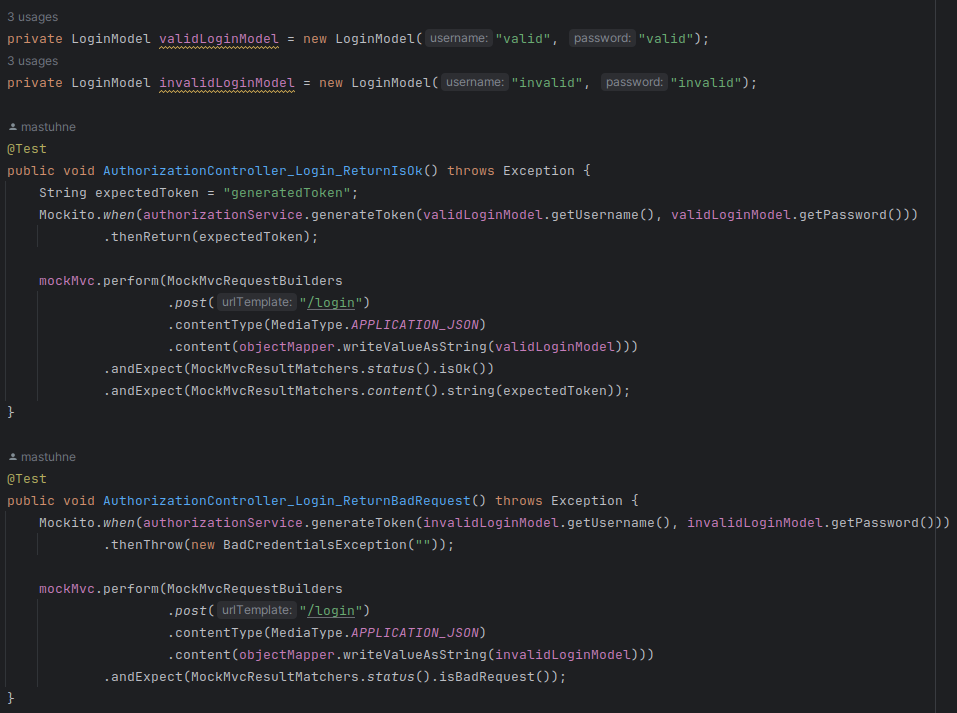
\includegraphics[scale=0.45]{slike/auth_controller_test.png}
				\centering
				\caption{AuthorizationControllerTest kod}
				\label{fig:authtest}
			\end{figure}

			\noindent\textbf{RecipeControllerTest}
			\begin{figure}[H]
				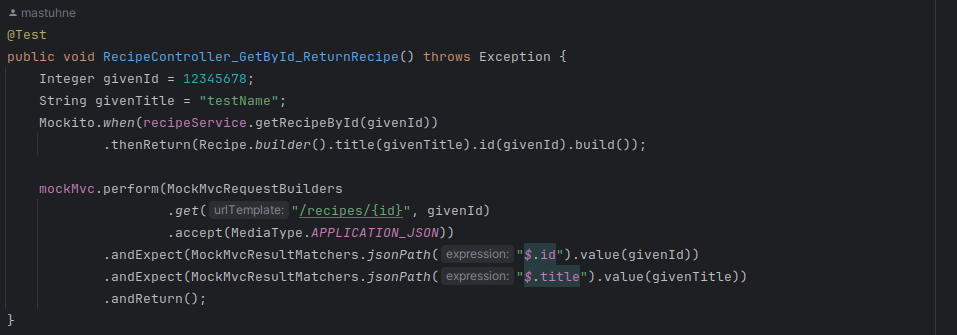
\includegraphics[scale=0.45]{slike/recipe_controller_test.png}
				\centering
				\caption{RecipeControllerTest kod}
				\label{fig:reccontrolltest}
			\end{figure}

			\eject
			\noindent\textbf{CategoryServiceTest}
			\begin{figure}[H]
				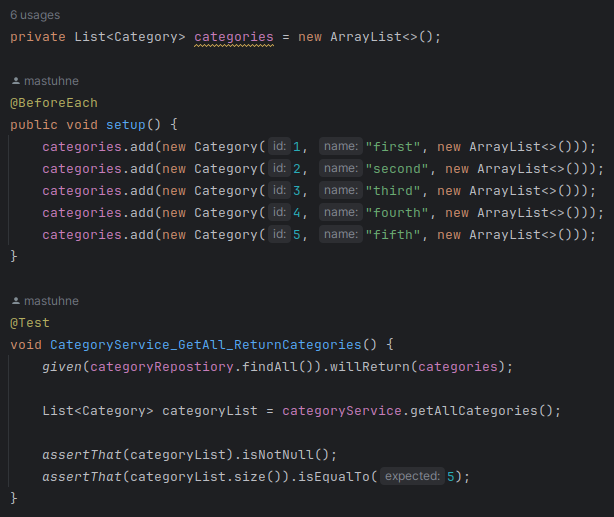
\includegraphics[scale=0.5]{slike/category_service_test.png}
				\centering
				\caption{CategoryServiceTest kod}
				\label{fig:cattest}
			\end{figure}

			\noindent\textbf{RecipeServiceTest}
			\begin{figure}[H]
				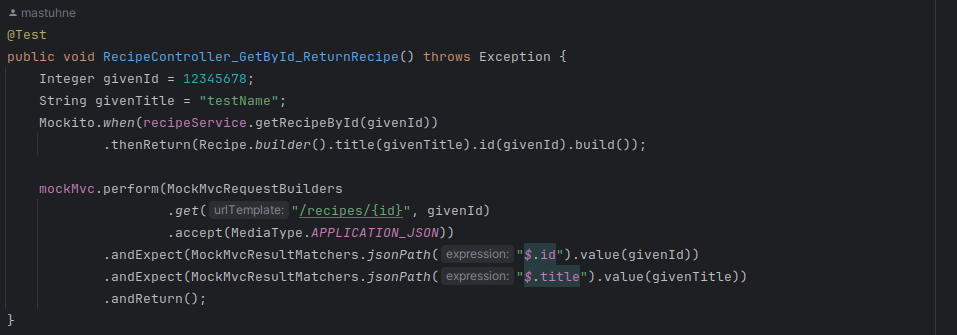
\includegraphics[scale=0.5]{slike/recipe_controller_test.png}
				\centering
				\caption{RecipeServiceTest kod}
				\label{fig:recest}
			\end{figure}

			\eject
			\noindent\textbf{UserRepositoryTest}
			\begin{figure}[H]
				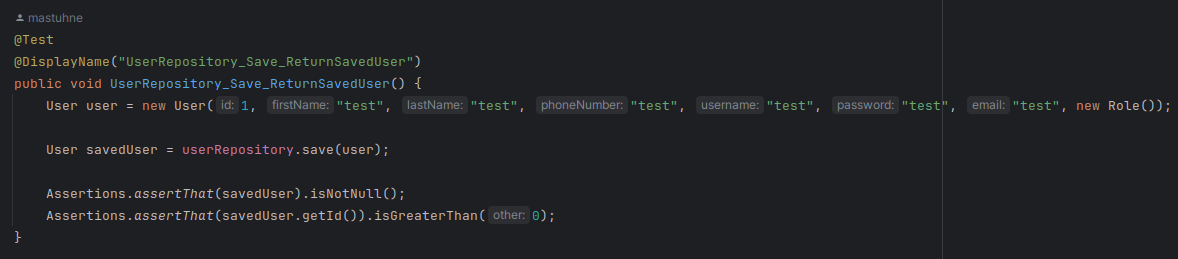
\includegraphics[scale=0.4]{slike/user_repository_test.png}
				\centering
				\caption{UserRepositoryTest kod}
				\label{fig:userretest}
			\end{figure}

			\noindent\textbf{Prikaz rezultata testova:}
			\begin{figure}[H]
				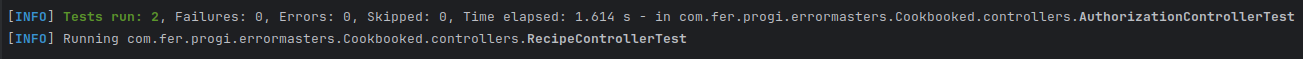
\includegraphics[scale=0.38]{slike/test_auth_con_res.png}
				\centering
				\caption{Rezultat AuthorizationControllerTest-a}
				\label{fig:authconres}
			\end{figure}
			\begin{figure}[H]
				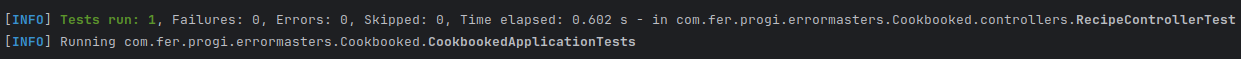
\includegraphics[scale=0.4]{slike/test_rec_con_res.png}
				\centering
				\caption{Rezultat UserRepositoryTest-a}
				\label{fig:recconres}
			\end{figure}
			\begin{figure}[H]
				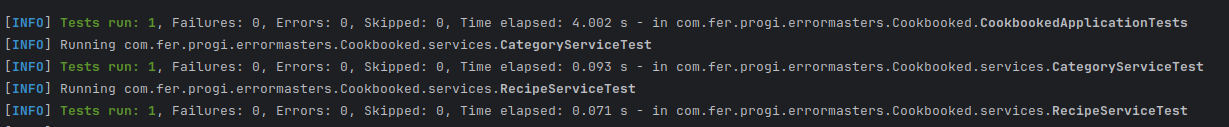
\includegraphics[scale=0.4]{slike/test_three_res.png}
				\centering
				\caption{Rezultat ... testa}
				\label{fig:threeres}
			\end{figure}
			\begin{figure}[H]
				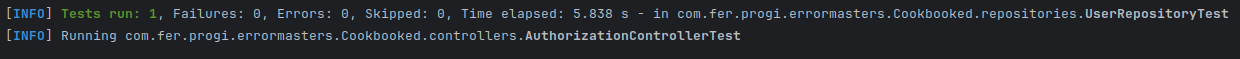
\includegraphics[scale=0.4]{slike/test_user_repo_res.png}
				\centering
				\caption{Rezultat UserRepositoryTest-a}
				\label{fig:userrepores}
			\end{figure}
			\begin{figure}[H]
				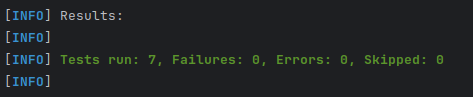
\includegraphics[scale=0.4]{slike/test_all_res.png}
				\centering
				\caption{Rezultat svih testova}
				\label{fig:allres}
			\end{figure}
			\eject




			
			\subsection{Ispitivanje sustava}
			
			 \textit{Potrebno je provesti i opisati ispitivanje sustava koristeći radni okvir Selenium\footnote{\url{https://www.seleniumhq.org/}}. Razraditi \textbf{minimalno 4 ispitna slučaja} u kojima će se ispitati redovni slučajevi, rubni uvjeti te poziv funkcionalnosti koja nije implementirana/izaziva pogrešku kako bi se vidjelo na koji način sustav reagira kada nešto nije u potpunosti ostvareno. Ispitni slučaj se treba sastojati od ulaza (npr. korisničko ime i lozinka), očekivanog izlaza ili rezultata, koraka ispitivanja i dobivenog izlaza ili rezultata.\\ }
			 
			 \textit{Izradu ispitnih slučajeva pomoću radnog okvira Selenium moguće je provesti pomoću jednog od sljedeća dva alata:}
			 \begin{itemize}
			 	\item \textit{dodatak za preglednik \textbf{Selenium IDE} - snimanje korisnikovih akcija radi automatskog ponavljanja ispita	}
			 	\item \textit{\textbf{Selenium WebDriver} - podrška za pisanje ispita u jezicima Java, C\#, PHP koristeći posebno programsko sučelje.}
			 \end{itemize}
		 	\textit{Detalji o korištenju alata Selenium bit će prikazani na posebnom predavanju tijekom semestra.}
			
			\eject 
		
		
		\section{Dijagram razmještaja}

			 \noindent Dijagram razmještaja prikazuje fizički razmještaj programskih artefakata 
			 na fizičkoj ili virtualnoj infrastrukturi. Na platformi DigitalOcean implementirano je
			 rješenje koje koristi Docker kontejnere za ispunjavanje pozadinske funkcionalnosti 
			 web aplikacije. Klijenti koriste web preglednik kako bi pristupili web applikaciji.
			 Sustav je baziran na arhitekturu "klijent-poslužitelj", dok je komunikacija između 
			 računala korisnika i računala poslužitelja ostvarena putem HTTP veze.
			

			\begin{figure}[H]
				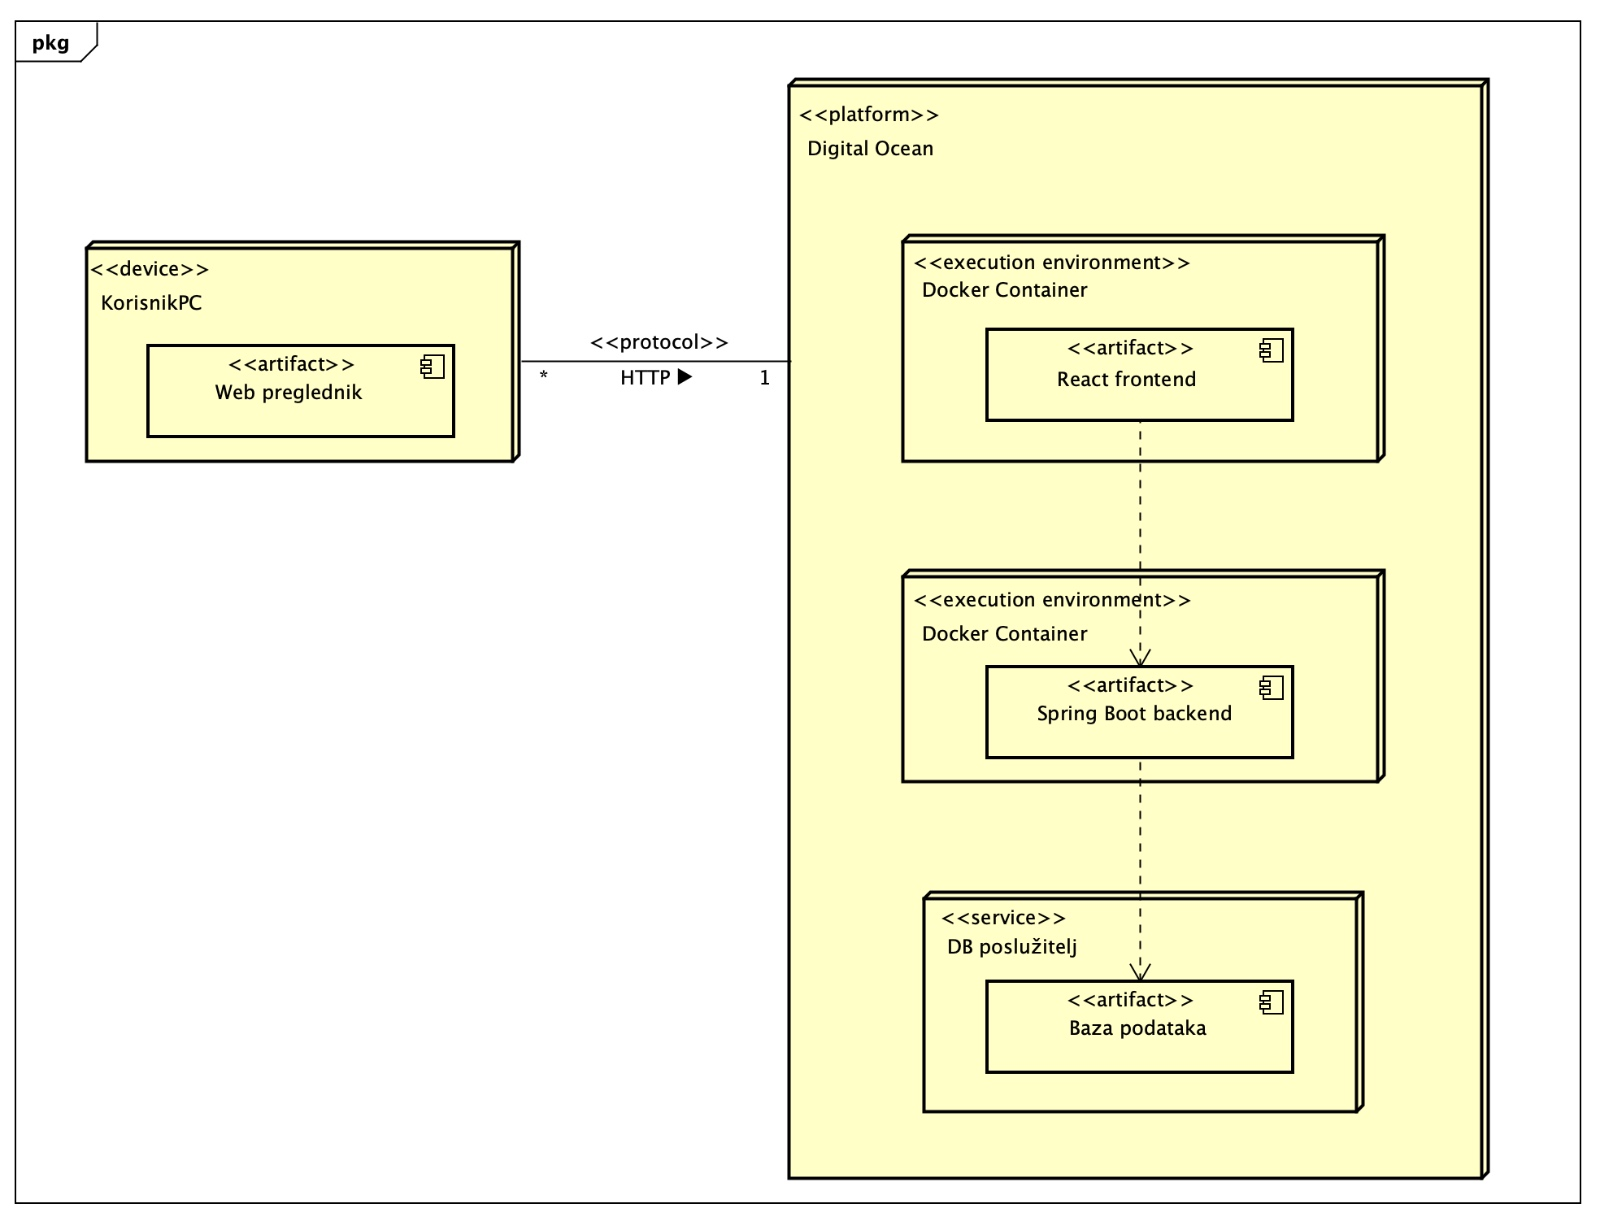
\includegraphics[scale=0.28]{dijagrami/dijagram_razmjestaja.jpeg}
				\centering
				\caption{Dijagram aktivnosti}
				\label{fig:bpdiag}
			\end{figure}
			\eject 
		
		\section{Upute za puštanje u pogon}
		
			\textbf{\textit{dio 2. revizije}}\\
		
			 \textit{U ovom poglavlju potrebno je dati upute za puštanje u pogon (engl. deployment) ostvarene aplikacije. Na primjer, za web aplikacije, opisati postupak kojim se od izvornog kôda dolazi do potpuno postavljene baze podataka i poslužitelja koji odgovara na upite korisnika. Za mobilnu aplikaciju, postupak kojim se aplikacija izgradi, te postavi na neku od trgovina. Za stolnu (engl. desktop) aplikaciju, postupak kojim se aplikacija instalira na računalo. Ukoliko mobilne i stolne aplikacije komuniciraju s poslužiteljem i/ili bazom podataka, opisati i postupak njihovog postavljanja. Pri izradi uputa preporučuje se \textbf{naglasiti korake instalacije uporabom natuknica} te koristiti što je više moguće \textbf{slike ekrana} (engl. screenshots) kako bi upute bile jasne i jednostavne za slijediti.}
			
			
			 \textit{Dovršenu aplikaciju potrebno je pokrenuti na javno dostupnom poslužitelju. Studentima se preporuča korištenje neke od sljedećih besplatnih usluga: \href{https://aws.amazon.com/}{Amazon AWS}, \href{https://azure.microsoft.com/en-us/}{Microsoft Azure} ili \href{https://www.heroku.com/}{Heroku}. Mobilne aplikacije trebaju biti objavljene na F-Droid, Google Play ili Amazon App trgovini.}
			
			
			\eject 